\documentclass[12pt,a4paper]{article}
\usepackage{amsmath}
\usepackage{amssymb}
\usepackage{listings}
\usepackage{xcolor}
\usepackage{graphicx}
\usepackage{hyperref}
\usepackage{tikz}
\usetikzlibrary{matrix,shadows}

% Define colors for code highlighting
\definecolor{codegreen}{rgb}{0,0.6,0}
\definecolor{codegray}{rgb}{0.5,0.5,0.5}
\definecolor{codepurple}{rgb}{0.58,0,0.82}
\definecolor{backcolour}{rgb}{0.95,0.95,0.92}

% Code listing style
\lstdefinestyle{mystyle}{
    backgroundcolor=\color{backcolour},   
    commentstyle=\color{codegreen},
    keywordstyle=\color{magenta},
    numberstyle=\tiny\color{codegray},
    stringstyle=\color{codepurple},
    basicstyle=\ttfamily\footnotesize,
    breakatwhitespace=false,         
    breaklines=true,                 
    captionpos=b,                    
    keepspaces=true,                 
    numbers=left,                    
    numbersep=5pt,                  
    showspaces=false,                
    showstringspaces=false,
    showtabs=false,                  
    tabsize=2
}

\lstset{style=mystyle}

\title{\textbf{Hardware project - Scientific Calculator}}
\author{EE24BTECH11012 - Bhavanisankar G S}
\date{\today}

\begin{document}

\maketitle

\begin{abstract}
This report presents the design and implementation of a scientific calculator using an Arduino UNO microcontroller. The calculator features a comprehensive set of mathematical functions including trigonometric, logarithmic, exponential operations, and numerical methods for solving differential equations. The implementation uses the Runge-Kutta 4th order method to compute various mathematical functions with high precision.
\end{abstract}

\tableofcontents

\section{Introduction}
The scientific calculator project aims to implement a wide range of mathematical functions on an Arduino UNO microcontroller with limited computational resources. Instead of relying on built-in math libraries, numerical methods have been implemented to compute functions like sine, cosine, logarithms, exponentials and inverse functions.

\section{Hardware Components}
\begin{itemize}
    \item Arduino UNO
    \item 16x2 LCD Display
    \item 20 push buttons to make 4x5 keypad
    \item Potentiometer
    \item Jumper wires
\end{itemize}

\begin{figure}[H]
	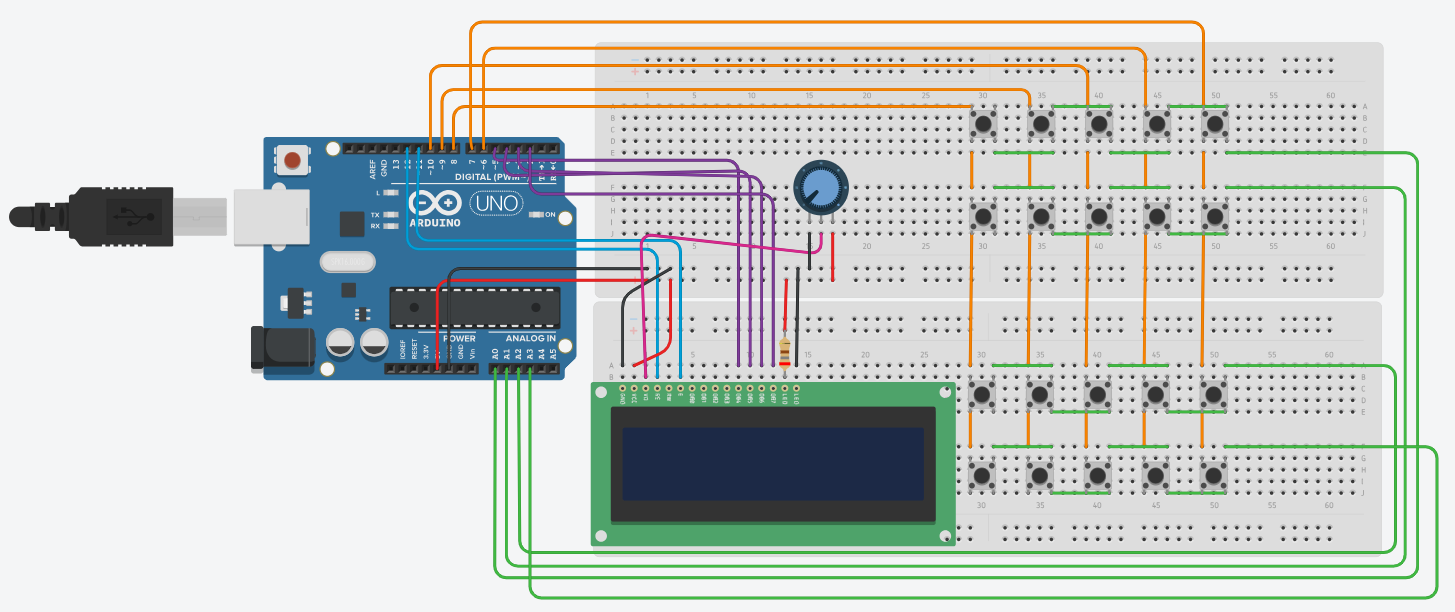
\includegraphics[width=\columnwidth]{figs/schematic.png}
	\caption{Schematic sketch}
	\label{Schematic}
\end{figure}

\subsection{LCD Interface}
The calculator uses a 16x2 LCD display in 4-bit mode with the following connections:

\begin{table}[h]
\centering
\begin{tabular}{|l|l|l|}
\hline
\textbf{LCD Pin} & \textbf{AVR Port/Pin} & \textbf{Arduino Pin} \\
\hline
Register Select (RS) & PORTD2 & 12 \\
\hline
Enable (EN) & PORTD3 & 11 \\
\hline
Data 4 (D4) & PORTD4 & 5 \\
\hline
Data 5 (D5) & PORTD5 & 4 \\
\hline
Data 6 (D6) & PORTD6 & 3 \\
\hline
Data 7 (D7) & PORTB4 & 2 \\
\hline
\end{tabular}
\caption{LCD Pin Connections}
\end{table}

\subsection{Keypad Interface}
A 4x5 matrix keypad is implemented with the following connections:

\begin{table}[h]
\centering
\begin{tabular}{|l|l|l|}
\hline
\textbf{Keypad} & \textbf{AVR Port/Pin} & \textbf{Arduino Pin} \\
\hline
Row 1 & PORTC0 & A0 \\
\hline
Row 2 & PORTC1 & A1 \\
\hline
Row 3 & PORTC2 & A2 \\
\hline
Row 4 & PORTC3 & A3 \\
\hline
Column 1 & PORTB0 & 8 \\
\hline
Column 2 & PORTB1 & 9 \\
\hline
Column 3 & PORTB2 & 10 \\
\hline
Column 4 & PORTD6 & 6 \\
\hline
Column 5 & PORTD7 & 7 \\
\hline
\end{tabular}
\caption{Keypad Matrix Connections}
\end{table}

\subsection{Keypad Layout}
The 4x5 keypad matrix has the following layout in normal mode:

\begin{table}[h]
\centering
\begin{tabular}{|c|c|c|c|c|}
\hline
7 & 8 & 9 & + & Del \\
\hline
4 & 5 & 6 & - & Shift \\
\hline
1 & 2 & 3 & * & Alpha \\
\hline
0 & . & = & / & Clr \\
\hline
\end{tabular}
\caption{Keypad Layout (Normal Mode)}
\end{table}

\section{User Interface}

\subsection{Input Modes}
The calculator supports three input modes:

\begin{enumerate}
    \item \textbf{Normal Mode}: Basic arithmetic and number entry
    \item \textbf{Shift Mode}: Access to inverse functions and special operations
    \item \textbf{Alpha Mode}: Access to scientific functions and constants
\end{enumerate}

The matrix design also supports these three different input modes without requiring additional hardware. This multiplexing technique allows a single button to have up to three different functions, effectively tripling the functionality without adding more hardware.

\subsection{Alpha Mode Functions}
In Alpha mode, the keypad provides access to scientific functions:

\begin{table}[h]
\centering
\begin{tabular}{|c|c|c|c|c|}
\hline
sin & cos & tan & \textasciicircum & BS \\
\hline
log & ln & e\textasciicircum & $\sqrt{x}$ & ( \\
\hline
$\pi$ & x^2 & x^3 & 1/x & ) \\

\hline
EXP & ANS & M+ & M- & MR \\
\hline
\end{tabular}
\caption{Keypad Layout (Alpha Mode)}
\end{table}

\subsection{Shift Mode Functions}
In Shift mode, the keypad provides access to additional functions:

\begin{table}[h]
\centering
\begin{tabular}{|c|c|c|c|c|}
\hline
asin & acos & atan & y\textasciicircum x & CLR \\
\hline
10\textasciicircum & e & abs & cbrt & [ \\
\hline
deg & rad & mod & fact & ] \\
\hline
HEX & DEC & BIN & OCT & MC \\
\hline
\end{tabular}
\caption{Keypad Layout (Shift Mode)}
\end{table}

\section{Mathematical Methods}
\subsection{Runge-Kutta 4th Order Method}
The Runge-Kutta 4th order method (RK4) is used to solve ordinary differential equations (ODEs). It provides a good balance between accuracy and computational complexity. For a first-order ODE of the form:

\begin{equation}
\frac{dy}{dx} = f(x, y)
\end{equation}

The RK4 method approximates the solution using:

\begin{align}
y_{n+1} &= y_n + \frac{1}{6}(k_1 + 2k_2 + 2k_3 + k_4) \\
k_1 &= h \cdot f(x_n, y_n) \\
k_2 &= h \cdot f(x_n + \frac{h}{2}, y_n + \frac{k_1}{2}) \\
k_3 &= h \cdot f(x_n + \frac{h}{2}, y_n + \frac{k_2}{2}) \\
k_4 &= h \cdot f(x_n + h, y_n + k_3)
\end{align}

where $h$ is the step size.

\subsection{Computing Trigonometric Functions}
Sine and cosine functions are computed by solving the second-order ODE:

\begin{equation}
\frac{d^2y}{dx^2} = -y
\end{equation}

This is converted to a system of first-order ODEs:

\begin{align}
\frac{dy_1}{dx} &= y_2 \\
\frac{dy_2}{dx} &= -y_1
\end{align}

With initial conditions:
\begin{itemize}
    \item For sine: $y_1(0) = 0, y_2(0) = 1$
    \item For cosine: $y_1(0) = 1, y_2(0) = 0$
\end{itemize}

\subsection{Computing Logarithmic Functions}
The natural logarithm is computed using the integral definition:

\begin{equation}
\ln(x) = \int_{1}^{x} \frac{1}{t} dt
\end{equation}

This is solved using the RK4 method with the differential equation:

\begin{equation}
\frac{dy}{dx} = \frac{1}{x}
\end{equation}

\subsection{Computing Exponential Functions}
The exponential function $e^x$ is computed by solving the ODE:

\begin{equation}
\frac{dy}{dx} = y
\end{equation}

With the initial condition $y(0) = 1$.

\section{Implementation Details}

\subsection{Code Structure}
The code is organized into several functional modules:
\begin{itemize}
    \item Numerical methods for mathematical functions
    \item LCD interface
    \item Keypad interface
    \item Expression parsing and evaluation
    \item Memory management
\end{itemize}



\subsection{User Interface}
The calculator provides three modes of operation:
\begin{itemize}
    \item Normal mode: Basic arithmetic operations
    \item Alpha mode: Scientific functions (sin, cos, log, etc.)
    \item Shift mode: Advanced functions (inverse trig, memory operations)
\end{itemize}

\section{Mathematical Functions}
The calculator implements the following mathematical functions:

\subsection{Trigonometric Functions}
\begin{itemize}
    \item $\sin(x)$: Computed using RK4 for the ODE $\frac{d^2y}{dx^2} = -y$ with initial conditions $y(0) = 0, y'(0) = 1$
    \item $\cos(x)$: Computed using RK4 for the ODE $\frac{d^2y}{dx^2} = -y$ with initial conditions $y(0) = 1, y'(0) = 0$
    \item $\tan(x)$: Computed as $\frac{\sin(x)}{\cos(x)}$
    \item $\sin^{-1}(x)$: Computed using numerical integration of $\frac{1}{\sqrt{1-x^2}}$
    \item $\cos^{-1}(x)$: Computed as $\frac{\pi}{2} - \sin^{-1}(x)$
    \item $\tan^{-1}(x)$: Computed using numerical integration of $\frac{1}{1+x^2}$
\end{itemize}

\subsection{Logarithmic and Exponential Functions}
\begin{itemize}
    \item $\ln(x)$: Computed using numerical integration of $\frac{1}{x}$
    \item $\log_{10}(x)$: Computed as $\frac{\ln(x)}{\ln(10)}$
    \item $e^x$: Computed using RK4 for the ODE $\frac{dy}{dx} = y$ with initial condition $y(0) = 1$
    \item $10^x$: Computed using the power function
\end{itemize}

\subsection{Power and Root Functions}
\begin{itemize}
    \item $\sqrt{x}$: Computed using RK4 for the ODE $\frac{dy}{dx} = \frac{1}{2y}$ with initial condition $y(1) = 1$
    \item $x^y$: Computed using iterative multiplication
    \item $\sqrt[3]{x}$: Computed using Newton's method
\end{itemize}

\subsection{Other Functions}
\begin{itemize}
    \item $|x|$: Absolute value
    \item $n!$: Factorial
    \item Degree-to-radian and radian-to-degree conversions
\end{itemize}

\subsection{Memory Functions}
The calculator includes memory operations:
\begin{itemize}
    \item Memory Recall (MR): Retrieve stored value
    \item Memory Add (M+): Add current value to memory
    \item Memory Subtract (M-): Subtract current value from memory
    \item Memory Clear (MC): Reset memory to zero
\end{itemize}

\section{Expression Evaluation}
The calculator parses and evaluates mathematical expressions following the BODMAS rule (Brackets, Orders, Division, Multiplication, Addition, Subtraction). The implementation handles:

\begin{itemize}
    \item Basic arithmetic operations: +, -, *, /, ^, %
    \item Function calls: sin(), cos(), log(), etc.
    \item Constants: π, e
    \item Memory operations: M+, M-, MR, MC
\end{itemize}

\section{Conclusion}
The scientific calculator implementation demonstrates how complex mathematical functions can be computed on resource-constrained microcontrollers using numerical methods. The Runge-Kutta method provides accurate approximations for differential equations, enabling the computation of transcendental functions without relying on built-in libraries. \\
The corresponding codes can be seen here - \\ \href{https://github.com/EE24BTECH11012/EE1003/tree/c55818859eebe407cd8a028f4a39012ec59f1942/Hardware/Calculator}{https://github.com/EE24BTECH11012/EE1003/Hardware/Calculator}

\end{document}

